\section{Modelo de vivienda}
\subsection{Dimensiones}

\begin{figure}[h] \centering
	\centering
	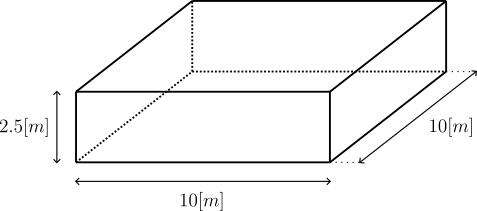
\includegraphics[width=1\textwidth]{./capitulos/resultados_discusion/images/modelo_vivienda.png}
	\caption{Vivienda modelo.}
	\label{fig:modelo_vivienda}
\end{figure}

Consideramos un modelo de vivienda simple con una única habitación de planta
cuadrada con $100[m^2]$ de área. Techo plano.

Las paredes son de $2.5[m]$ de alto, por lo tanto con una extesión total de
$100[m^2]$. De los cuales 25 son ventanas y los otros 75 son pared.

El volumen es de $100[m^2] \cdot 2.5[m] = 250[m^3]$, con
tan solo aire en su interior, que tiene una densidad de
$1.1614[kg \cdot m^{-3}]$, y pesará:

\begin{equation}
	m_{aire} = 1.1614 \cdot 250 = 290.35[kg]
\end{equation}



\subsection{Transmitancias térmicas de la vivienda}

La transmitancia térmica de las ventanas se extrae de la ficha técnica para un
modelo
\footnote{\url{https://www.veka.es/wp-content/uploads/2020/03/softline-70-doble-junta-linea-recta-por-paginas.pdf}},
que muestra (figura \ref{fig:window_tranmittance}) sus medidas de transmitancia
para el marco (frame), vidrio (glass) y global (window). Escogiendo el vidrio
de baja emisividad (BE) y relleno de argón, tenemos un valor de
$1.4\left[\frac{W}{m^2 \cdot K}\right]$, que asumimos engloba las perdidas por
conducción, convección y radiación.

\begin{figure}[h] \centering
	\centering
	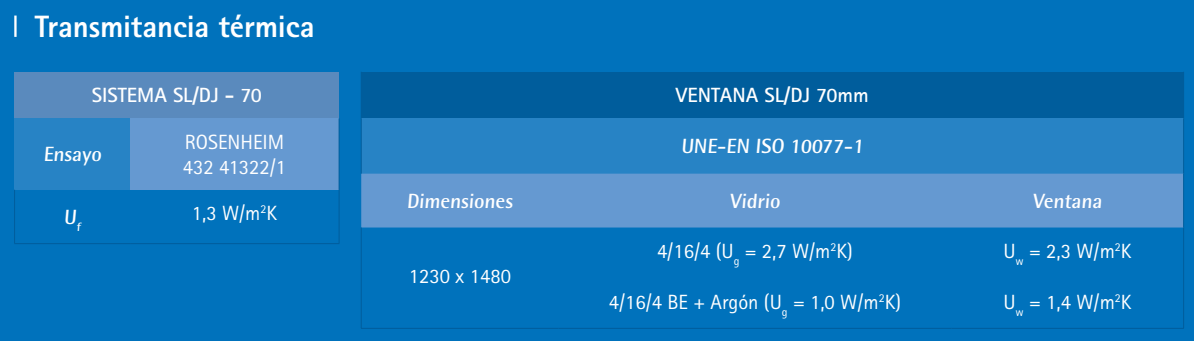
\includegraphics[width=1\textwidth]{./capitulos/resultados_discusion/images/window_transmittance.png}
	\caption{Transmitancias térmicas para ventana Veka softline 70.}
	\label{fig:window_tranmittance}
\end{figure}


Tanto paredes como techo tienen un aislamiento de $20[cm]$ de espesor de lana
de roca. Y con el dato de la conductividad térmica de este material obtenida de
la tabla de propiedades físicas en Incropera et al.
\cite{incropera1996fundamentals}, se calcula la transmitancia térmica por
conducción de un metro cuadrado de este aislamiento como


\begin{equation}
	U_{lana-roca} = \frac{k}{l} = \frac{0.049\left[\frac{W}{m \cdot K}\right]}{0.2[m]} = 0.245 \left[\frac{W}{m^2 \cdot K}\right]
\end{equation}

Pero además de pérdidas por conducción, consideramos la transferencia por
convección y radiación, tomando los datos para una superficie no reflejante
(con emisividad de 0.9) de la tabla \ref{tab:building_surface_transmittances}
obtenida de ASHRAE \cite{refrigerating2009ashrae}.

\begin{table}[ht]
	\centering
	\caption{Resistencia y conductancia para aire y superficies de edificios con $\epsilon = 0.9$}
	\label{tab:building_surface_transmittances}
	\begin{tabular}{llcc}
		\toprule
		\textbf{Position of Surface}       & \textbf{Direction of Heat Flow} & $h_i$ & $R$   \\
		\midrule
		\textbf{Still Air}                 &                                 &       &       \\
		Horizontal                         & Upward                          & 9.26  & 0.11  \\
		Sloping at 45°                     & Upward                          & 9.09  & 0.11  \\
		Vertical                           & Horizontal                      & 8.29  & 0.12  \\
		Sloping at 45°                     & Downward                        & 7.50  & 0.13  \\
		Horizontal                         & Downward                        & 6.13  & 0.16  \\
		\midrule
		\textbf{Moving Air (any position)} &                                 &       &       \\
		Wind (for winter) at 6.7 m/s       & Any                             & 34.0  & 0.030 \\
		Wind (for summer) at 3.4 m/s       & Any                             & 22.7  & 0.044 \\
		\bottomrule
	\end{tabular}
\end{table}


Con estos datos calculamos las transmitancias de paredes y techo como:

\begin{equation}
	\frac{1}{U} = \frac{1}{h_{pared-interior}} + \frac{1}{U_{lana-roca}} + \frac{1}{h_{pared-exterior}}
\end{equation}

tomando como $h_{pared-exterior}$ la media entre los dos datos dados, de verano
e invierno:

\begin{equation}
	\frac{1}{U_{paredes}} = \frac{1}{8.29} + \frac{1}{0.245} + \frac{1}{28.35} \rightarrow U_{paredes} = 0.2359 \left[\frac{W}{m^2 \cdot K}\right]
\end{equation}

\begin{equation}
	\frac{1}{U_{techo}} = \frac{1}{9.26} + \frac{1}{0.245} + \frac{1}{28.35} \rightarrow U_{techo} = 0.2366 \left[\frac{W}{m^2 \cdot K}\right]
\end{equation}


\subsection{Suelo radiante}

Por simplicidad, consideramos un único circuito con tubo de polietileno reticulado (PEX) de 1
pulgada que lleva unas dimensiones asociadas mostradas en la figura
\ref{fig:1_inch_pex}.
Aunque en la práctica es más común la instalación de varios circuitos (e.g.
uno para cada habitación), cada uno con diámetros de tubo menores.

\begin{figure}[h] \centering
	\centering
	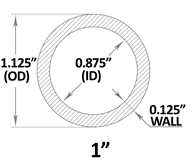
\includegraphics[width=0.3\textwidth]{./capitulos/resultados_discusion/images/1_inch_pex.png}
	\caption{Dimensiones de un tubo PEX de una pulgada. Fuente: \url{https://www.pexuniverse.com/pex-tubing-technical-specs}.}
	\label{fig:1_inch_pex}
\end{figure}


Para el espaciado entre pasos de tubo, se adopta una convención establecida
\footnote{\url{https://www.blueridgecompany.com/articles/PEX_tube_sizing_spacing}},
seleccionando una distancia de 18" (redondeando a $50[cm]$) entre pasos. La
configuración en zig-zag permite determinar la longitud total del tubo (figura
\ref{fig:esquema_tubos_suelo}). Que puede observarse es de $H = 21 \cdot 10 + 10 =
220[m]$.

Y el área de los tubos viene dada por la longitud total de estos $H$, y el
perímetro exterior del tubo.

\begin{equation}
	A_{tubos} = 2 \pi R_{ext} H = 2 \pi \cdot 0.0142875 \cdot 220 = 19.7[m^2]
\end{equation}


\begin{figure}[h] \centering
	\centering
	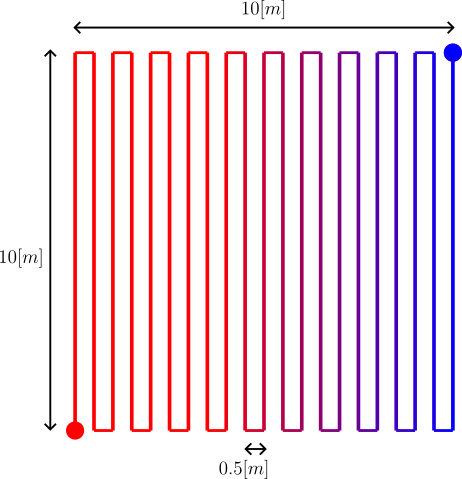
\includegraphics[width=0.6\textwidth]{./capitulos/resultados_discusion/images/esquema_tubos_suelo.png}
	\caption{Suelo radiante, configuración zig-zag. 220 metros de longitud.}
	\label{fig:esquema_tubos_suelo}
\end{figure}

De nuevo hemos optado por un arreglo simple para facilitar los cálculos,
pero también es común el patrón de espiral, mostrado en la figura \ref{fig:spiral_pattern_floor},
que distribuye el calor de forma más uniforme por el suelo, aunque con una buena
conductividad del material de la losa que integra los tubos (hormigón), las diferencias de
temperaturas en distintas partes de la habitación deberían de ser poco perceptibles.

\begin{figure}[h] \centering
	\centering
	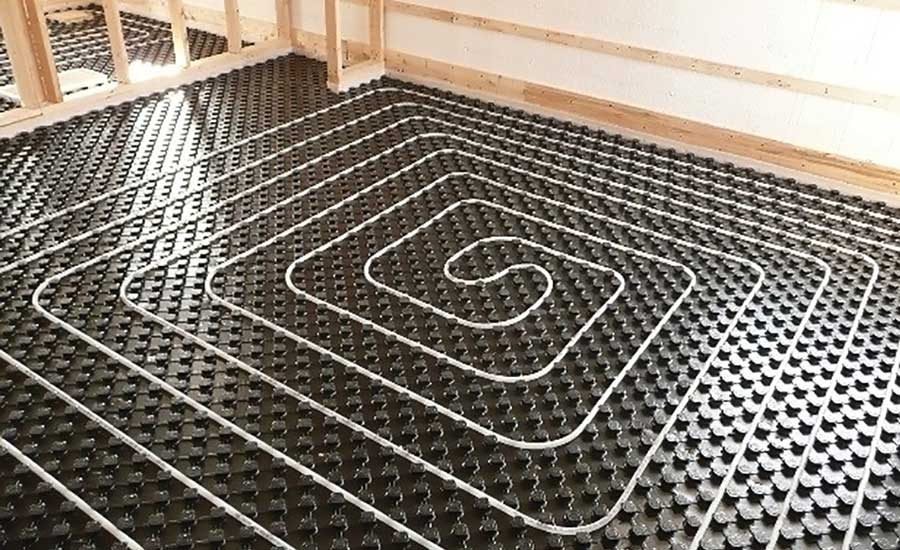
\includegraphics[width=1\textwidth]{./capitulos/resultados_discusion/images/spiral_pattern_floor.jpg}
	\caption{Tubos para suelo radiante en configuración espiral. Fuente: \url{https://www.achrnews.com/articles/141245-hydronics-offer-unique-options-for-residential-heating}.}
	\label{fig:spiral_pattern_floor}
\end{figure}

La losa de hormigón que da una inercia térmica considerable al suelo, se ha
tomado de 5cm. Y tampoco hemos considerado que se haya recubierto la losa de
hormigón con ningún azulejo, porcelánico o madera.

Con una densidad del hormigón de $2300[kg\cdot m^{-3}]$, la masa de esta losa es:

\begin{equation}
	m_{suelo} = 100[m^2] \cdot 0.05[m] \cdot 2300[kg\cdot m^{-3}] = 11500[kg]
\end{equation}


\subsection{Paneles solares}

Ya que disponemos de un techo de $100[m^2]$, y cada kW de paneles solares
requiere de un área de aproximadamente $5[m^2]$, como se muestra en el SAM
(figura \ref{fig:solar_panel_area}), como mucho podremos instalar $20[kW]$ de
potencia solar.

\begin{figure}[h] \centering
	\centering
	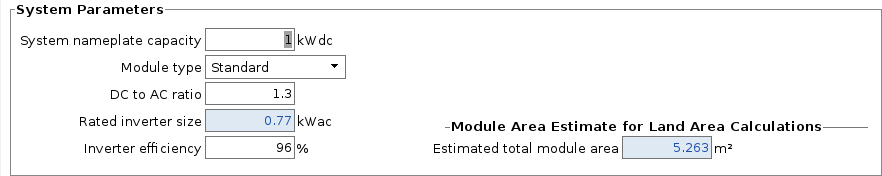
\includegraphics[width=1\textwidth]{./capitulos/resultados_discusion/images/solar_panel_area.png}
	\caption{Área de $5.263[m^2]$ para $1[kW]$ de panales solares instalados. Datos obtenidos de SAM (System Advisor Model).}
	\label{fig:solar_panel_area}
\end{figure}


\subsection{Tanque de agua}

Tiene forma cilíndrica con misma altura que diámetro (figura
\ref{fig:water_tank}), y su masa y superficie son función del volumen.

\begin{figure}[h] \centering
	\centering
	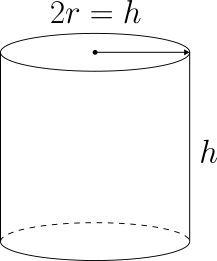
\includegraphics[width=0.2\textwidth]{./capitulos/resultados_discusion/images/water_tank.png}
	\caption{Depósito de agua caliente.}
	\label{fig:water_tank}
\end{figure}

\begin{align} \label{eq:tank_mass_and_area}
	V_{tanque} & = \pi r^2 h = 2 \pi r^3 \rightarrow r = \sqrt[3]{\frac{V_{tanque}}{2\pi}} \\
	m_{tanque} & = V_{tanque} \cdot \rho_{agua} \\
	A_{tanque} & = 2 \pi r \cdot h
\end{align}

\clearpage

\section{Sistema eléctrico}
\begin{figure}[h] \centering
	\centering
	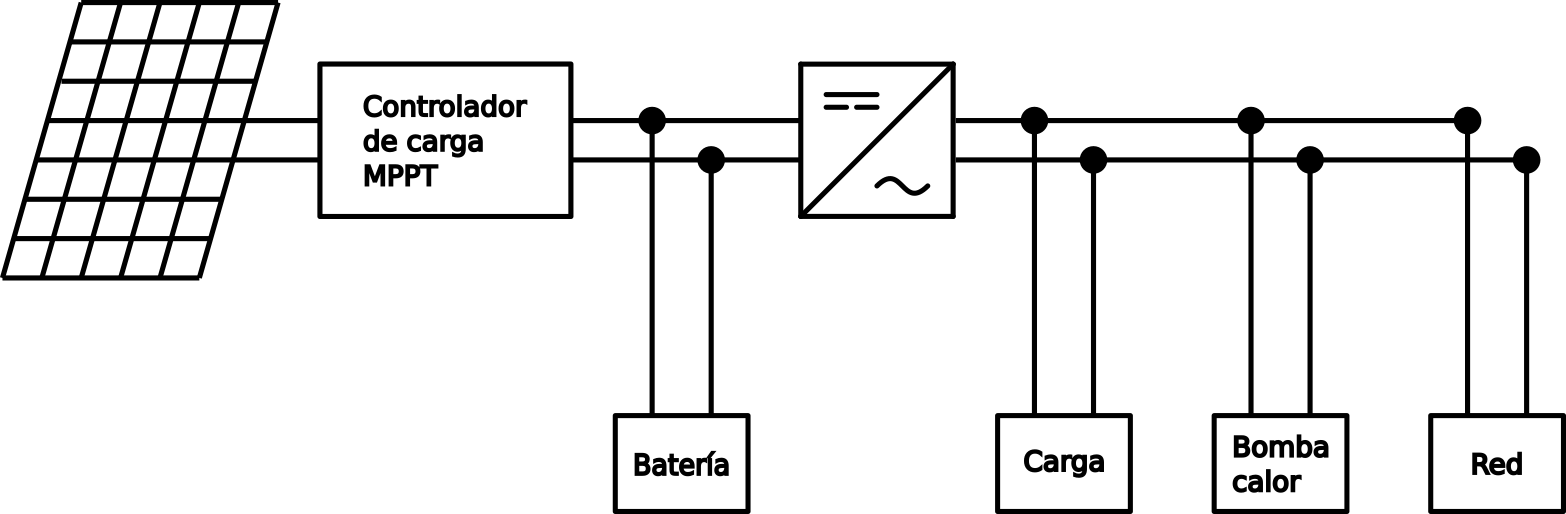
\includegraphics[width=1\textwidth]{./capitulos/resultados_discusion/images/diagrama_electrico.png}
	\caption{Diagrama eléctrico.}
	\label{fig:electic_diagram}
\end{figure}

Tenemos un sistema con paneles fotovoltaicos conectados a un controlador de
carga MPPT (Maximum Power Point Tracking) que con un controlador de electrónica
de potencia regula la tensión de salida de los paneles para obtener el máximo
de potencia en la curva P-V (figura \ref{fig:solar_P-V_I-V}) a través de algún
algoritmo, como el 'Perturb and Observe' (P\&O), donde se actualiza el valor de
la tensión de referencia con el gradiente de la potencia respecto a la tensión.

\begin{equation}
	V_{k} \leftarrow V_k + \alpha \frac{P_k - P_{k-1}}{V_{k}-V_{k-1}}
\end{equation}

\begin{figure}[h] \centering
	\centering
	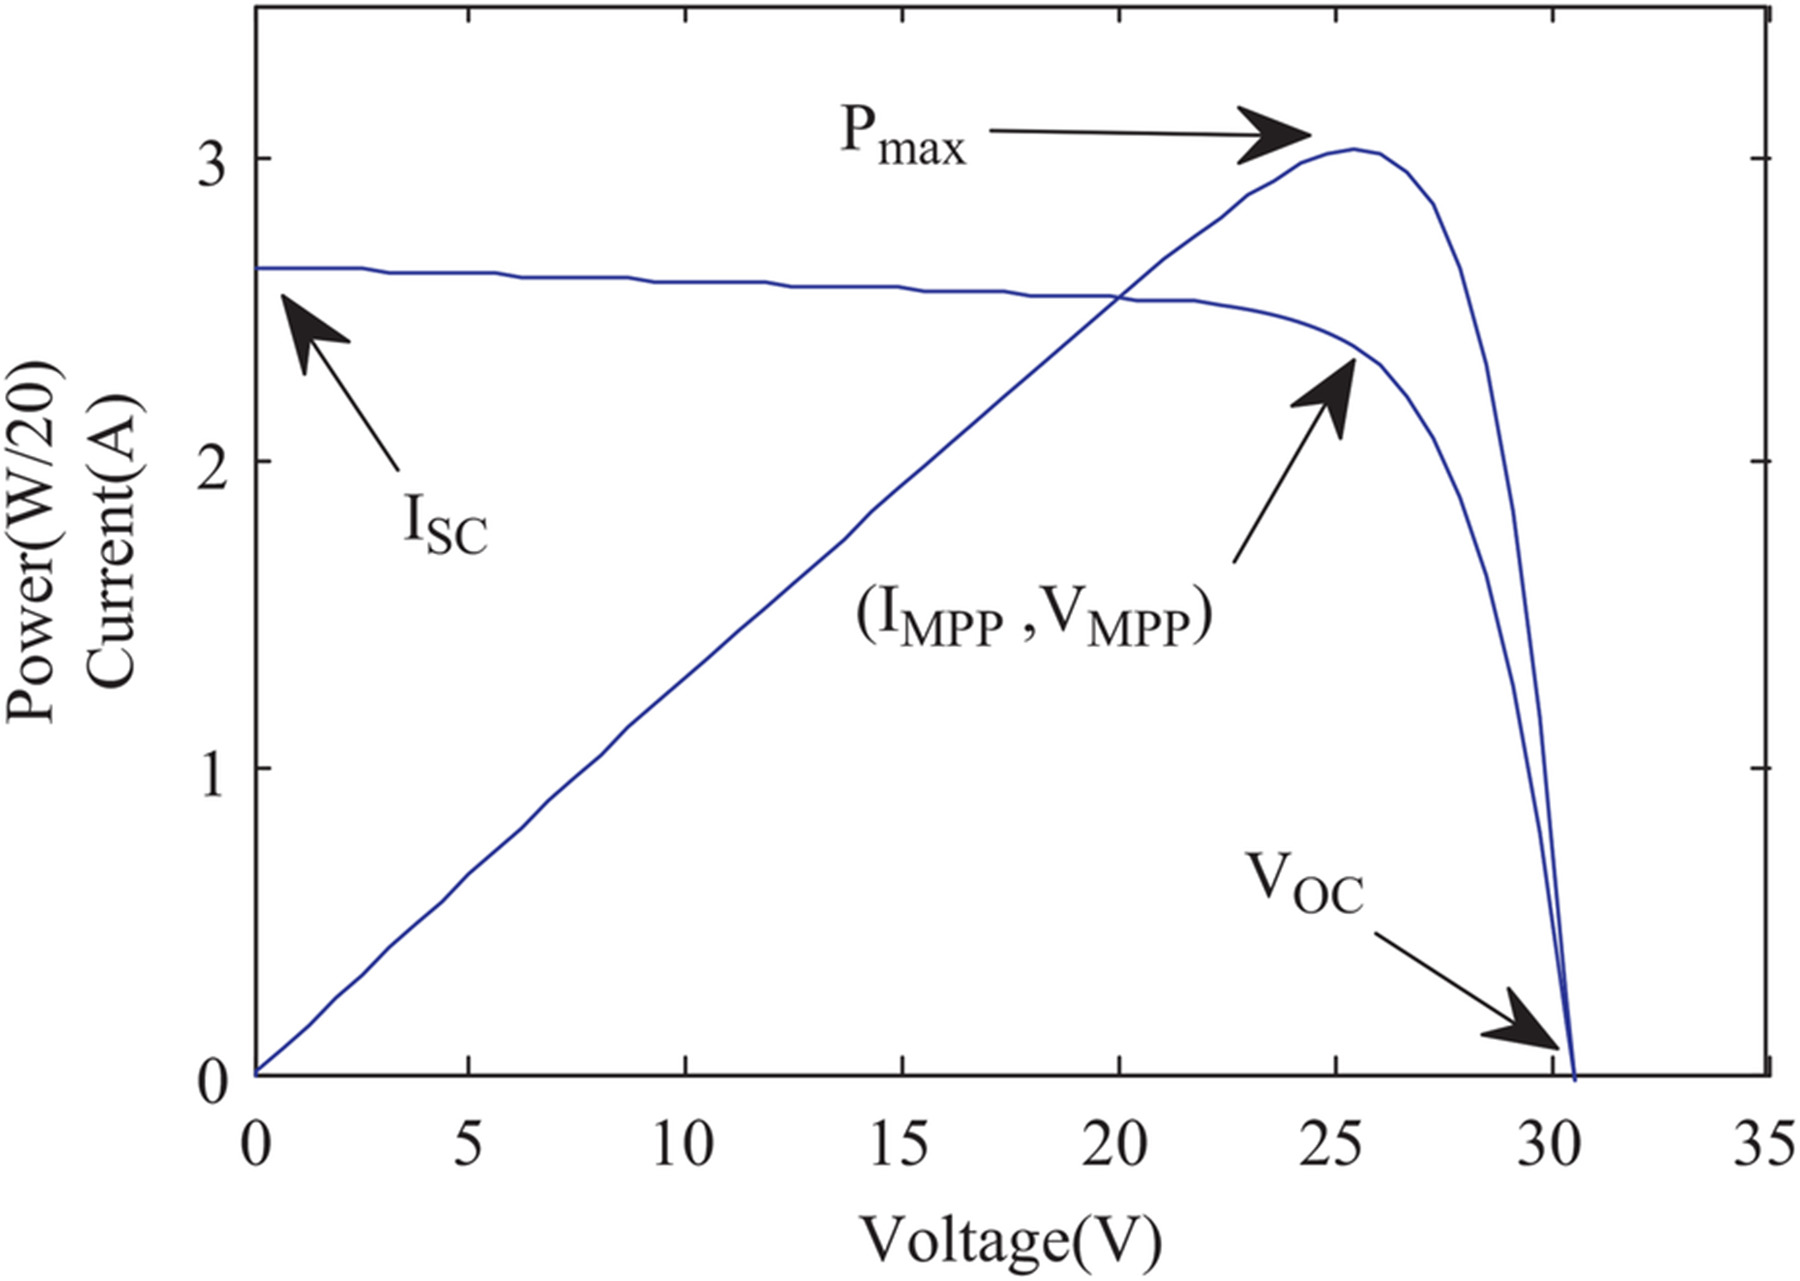
\includegraphics[width=0.6\textwidth]{./capitulos/resultados_discusion/images/solar_P-V_I-V.jpg}
	\caption{Curvas P-V e I-V para un panel solar \cite{podder2019mppt}.}
	\label{fig:solar_P-V_I-V}
\end{figure}


La batería elegida es de tipo LiFePO4 (litio-ferrofosfato) que es comunmente
empleada en aplicaciones de almacenamiento energético. Con tensión nominal total
de 48V.

Conectado al lado de alterna a través de un convertidor DC/AC bidireccional,
donde tenemos la demanda de energía del domicilio (carga), la potencia
destinada a la bomba de calor (compresor), y finalmente está la red, de donde
podemos obtener o volcar energía. Por lo general los precios de compra y venta
son distintos, y así hemos reflejado, usando el precio de mercado diario como
el precio de venta de excedentes, y PVPC (Precio Voluntario para el Pequeño
Consumidor) como el precio de compra, que es mayor que el anterior al incluir
peajes y cargos regulatorios.

En caso de funcionamiento off-grid, reemplazamos la red por un generador diesel
con un precio fijo del combustible, e imponiendo la restricción de que no
podemos volcar energía a este.


Tomando todas las potencias en alterna, el balance energético de esta
instalación queda reflejado por:

\begin{equation}
	P_{red} + P_{solar} = P_{carga} + P_{bat} + P_{bomba}
\end{equation}

donde se han tomado como positivas las potencias de entrada al nodo, y potencia
positiva positiva para la red en caso de demandar energía de esta, y para la
batería cuando se está cargando. Como se refleja en la figura
\ref{fig:electric_node}

\begin{figure}[h] \centering
	\centering
	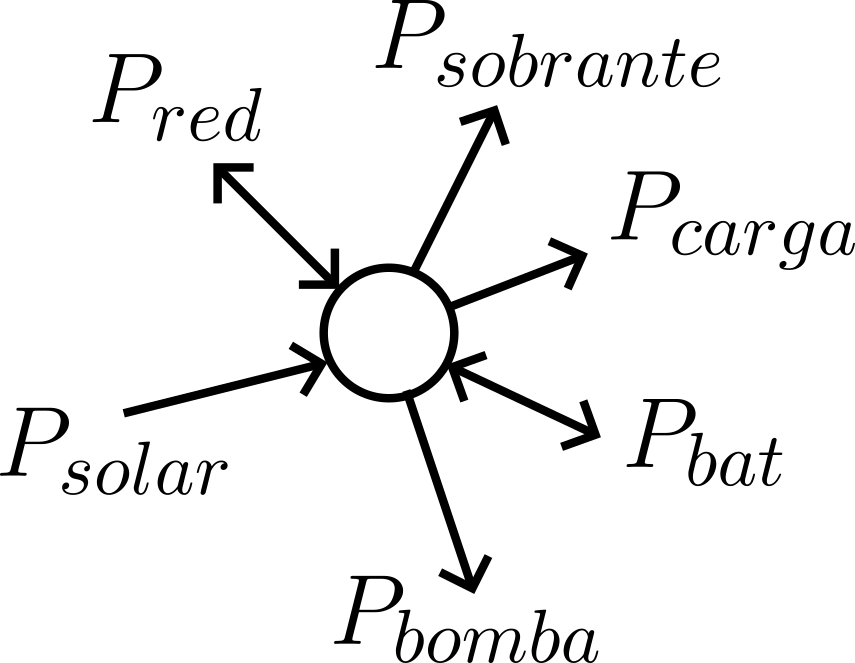
\includegraphics[width=0.4\textwidth]{./capitulos/resultados_discusion/images/electric_node.png}
	\caption{Balance de potencias eléctricas.}
	\label{fig:electric_node}
\end{figure}

La dinámica de las baterías corresponde a

\begin{equation}
	\frac{de}{dt} = \mu_{bat} P_{bat}
\end{equation}

donde $e$ es la energía almacenada, $P_{bat}$ la potencia de alimentación a la
batería y $\mu_{bat}$ la eficiencia de conversión desde alterna a energía
almacenada.

Y a esta le aplicamos las restricciones para los niveles de carga máximo y
mínimo, SOC (State Of Charge)

\begin{equation}
	\text{SOC} = \frac{e}{e_{max}}
\end{equation}

\begin{equation}
	\text{SOC}_{min} \leq \text{SOC} \leq \text{SOC}_{max}
\end{equation}

donde $e_{max}$ es la capacidad, o energía máxima que puede acumular la batería.

Aplicamos como condición inicial que esté en su punto mínimo de carga, partimos
de que está 'vacía'

\begin{equation}
	e_0 = e_{max} \text{SOC}_{min}
\end{equation}

Y la potencia máxima con la que podemos cargar o descargar es función de la capacidad,
a través del factor C-rate, que para células de LiFePO4 establecimos era de aproximadamente
0.3 el valor recomendado, mientras que el máximo nominal de contínuo funcionamiento era de 1.

Podemos relacionar la capacidad y potencia máxima, primero sabiendo que
el C-rate se define como la relación entre la corriente máxima y la capacidad en amperios-hora

\begin{equation}
  i_{max}[A] = \text{C}[Ah] \text{C-rate}
\end{equation}

y luego multiplicando ambos miembros por la tensión nominal

\begin{align}
  i_{max}[A] \, v[V] &= v[V] \, \text{C}[Ah] \, \text{C-rate} \\
  P_{bat_{max}} &= e[Wh] \, \text{C-rate}
\end{align}

Cuando tratemos de sacar las dimensiones optimas de baterías, bomba de calor y
potencia contratada de red, tendremos como variables de diseño la capacidad de
la batería (de donde sacamos la potencia máxima de la batería), y potencía
máxima del compresor y de red respectivamente.

Y estos valores máximos los aplicaremos como restricciones para las variables
de control $P_{bat}$, $P_{red}$ y $P_{bomba}$.

\begin{align}
  -P_{bat_{max}} < P_{bat} < P_{bat_{max}} \\
  -P_{red_{max}} < P_{red} < P_{red_{max}} \\
  0 < P_{bomba} < P_{bomba_{max}}
\end{align}


\section{Sistema térmico}
\begin{figure}[h] \centering
	\centering
	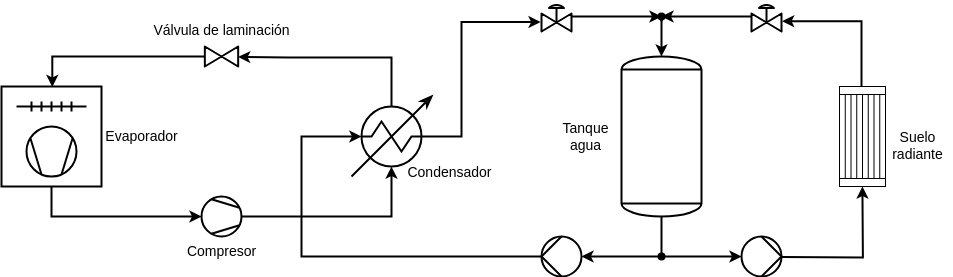
\includegraphics[width=1\textwidth]{./capitulos/resultados_discusion/images/sistema_termico.png}
	\caption{Esquema térmico.}
	\label{fig:thermal_diagram}
\end{figure}

Una bomba de calor produce agua caliente sanitaria que se almacena en un
depósito acumulador. De este se extraen dos flujos, uno de vuelta al
intercambiador de calor del condensador de la bomba de calor
($\dot{m}_{cond}$), y otro que se dirige al suelo radiante ($\dot{m}_{cale}$).

Estos dos caudales se controlan a través de dos bombas de circulación y
posiblemente también mediante válvulas de estrangulación, si las bombas no
fueran de velocidad variable (VFD, Variable Frequency Drive).

La temperatura del tanque de agua es $T_{tanque}$, a la salida de la calefacción
del suelo radiante $T_{cale}$, y a continuación del condensador $T_{cond}$.

\subsection{Bomba de calor}

En lugar de modelar detalladamente la bomba de calor con sus componentes
(evaporador, compresor, condensador y válvula de expansión), se ha optado por
aproximar el COP (Coeficiente de Rendimiento) utilizando datos de hojas
técnicas. El COP se expresa en función de la temperatura de salida del agua del
condensador, denominada $T_{cond}$.

Según los datos de una bomba de calor comercial
\footnote{\url{https://www.daikin.es/content/dam/DACS/document-library/Pdfs-subidos-2022/Monobloc\%20EBLA\%209-11\%20-\%2014-16.pdf}}
el COP es 4.8 para una temperatura de 35°C y 3.4 para 55°C. Se ha considerado
una variación lineal del COP entre estos puntos, con un valor mínimo de 0 y un
máximo de 4.8.

La función por partes que describe el COP es:

\begin{equation}
	\text{\text{cop}}(T) =
	\begin{cases}
		4.8              & \text{si } T < 35^\circ C                    \\[10pt]
		26.36 - 0.069 T & \text{si } 35^\circ C \leq T < 103.5^\circ C \\[10pt]
		0                & \text{si } T \geq 103.5^\circ C
	\end{cases}
\end{equation}

que se muestra en la figura \ref{fig:heat_pump_cop}

\begin{figure}[h] \centering
	\centering
	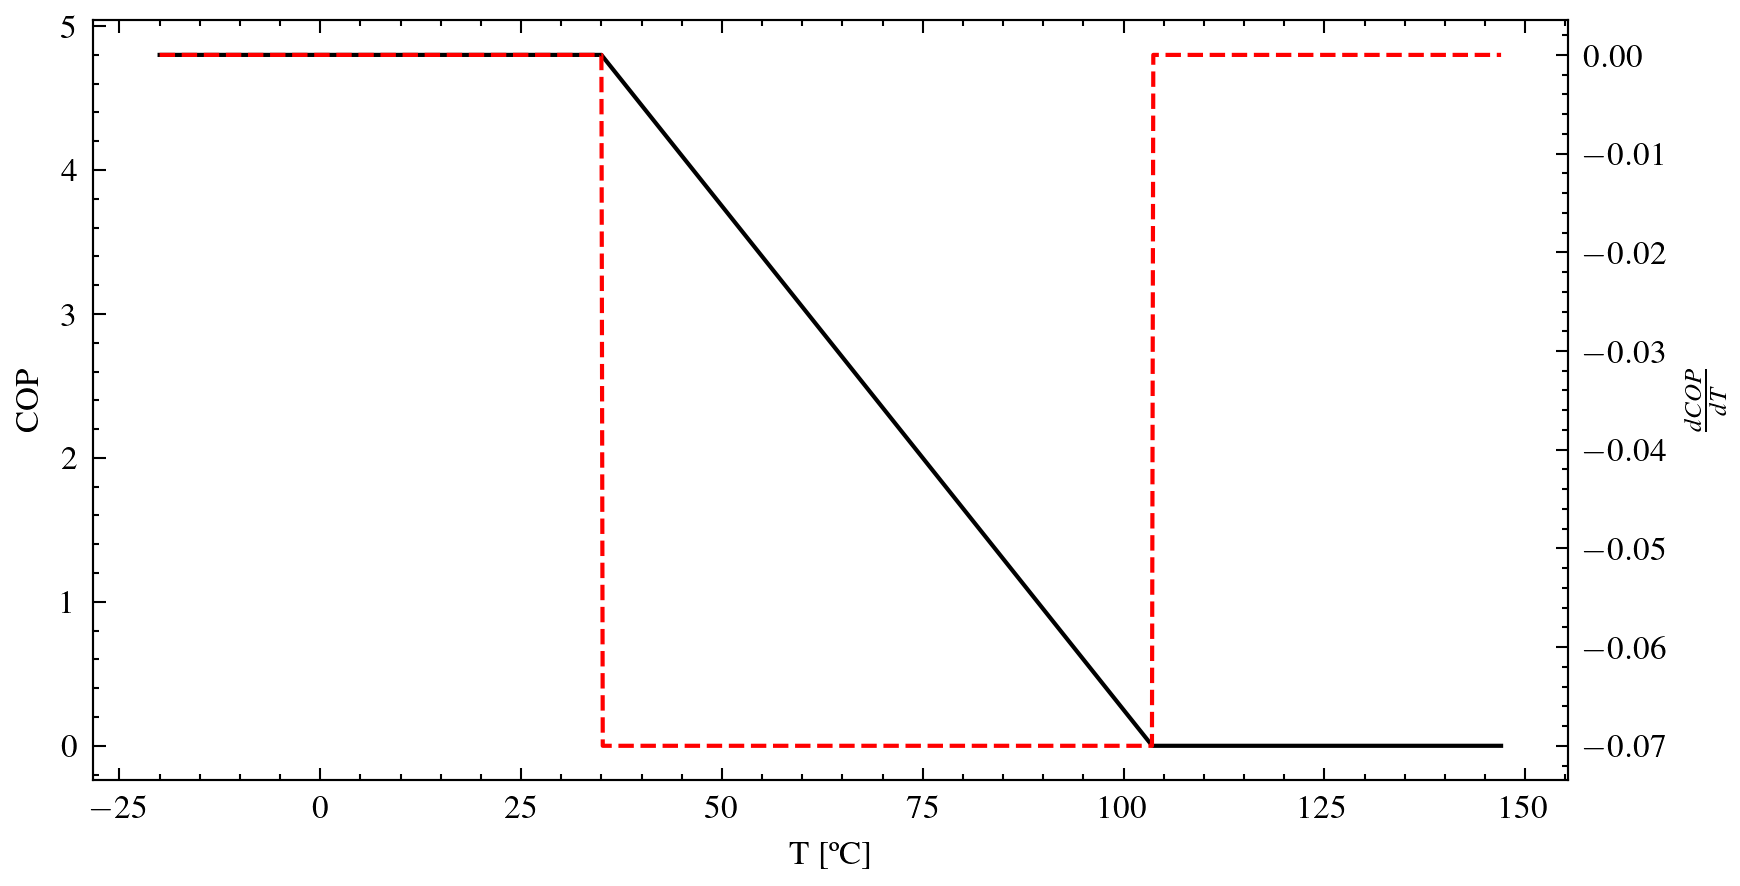
\includegraphics[width=1\textwidth]{./capitulos/resultados_discusion/images/heat_pump_cop.png}
	\caption{COP de la bomba de calor según la temperatura de salida del agua.
		Eje de ordenadas derecho muestra la derivada del COP respecto de la
		temperatura.}
	\label{fig:heat_pump_cop}
\end{figure}


\subsection{Tanque de agua}

Desde el depósito de agua aislado térmicamente, tenemos dos flujos de entrada y
salida controlados por dos bombas de circulación. Un caudal para la bomba de
calor $\dot{m}_{cond}$, y otro para el suelo radiante $\dot{m}_{suelo}$.

La ecuación de conservación de la energía para el tanque con pérdidas de calor
por conducción con el ambiente (suponemos que se encuentra en el exterior de la
vivienda) es

\begin{align} \label{eq:t_tanque_balance}
	m_{tanque} \cdot cp_{agua} \cdot \left( \frac{dT_{tanque}}{dt} \right) & = \dot{m}_{cond} \cdot cp_{agua} \cdot T_{cond} \nonumber     \\
	                                                                       & + \dot{m}_{cale} \cdot cp_{agua} \cdot T_{cale} \nonumber     \\
	                                                                       & - \dot{m}_{tanque} \cdot cp_{agua} \cdot T_{tanque} \nonumber \\
	                                                                       & - \dot{Q}_{perdida}
\end{align}

con las ecuaciones

\begin{align}
	\text{COP}        & = \text{cop}(T_{cond})         \label{eq:cop_t_cond}                               \\
	\dot{Q}_{cond}    & = \text{COP} \cdot P_{bomba}   \label{eq:q_cond_1}                                 \\
	\dot{Q}_{cond}    & = \dot{m}_{cond} \cdot cp_{agua} \cdot (T_{cond} - T_{tanque}) \label{eq:q_cond_2} \\
	\dot{m}_{tanque}  & = \dot{m}_{cond} + \dot{m}_{cale}      \label{eq:m_dot_tanque}                     \\
	\dot{Q}_{perdida} & = U_{tanque} \cdot A_{tanque} \cdot (T_{tanque} - T_{amb})  \label{eq:q_perdida}
\end{align}

donde

\begin{itemize}
	\item $\text{COP}$: Coeficiente de rendimiento.
	\item $\text{cop}(T_{cond})$: Función que define el COP en función de $T_{cond}$.
	\item $m_{tanque}$: Masa del tanque.
	\item $cp_{agua}$: Calor específico del agua.
	\item $\dot{m}_{tanque}$: Flujo másico del tanque.
	\item $\dot{m}_{cond}$: Flujo másico del condensador.
	\item $\dot{m}_{cale}$: Flujo másico de suelo radiante, calefacción.
	\item $T_{tanque}$: Temperatura del tanque.
	\item $T_{cond}$: Temperatura a la salida el condensador.
	\item $T_{cale}$: Temperatura calefacción, a la salida del suelo radiante.
	\item $T_{amb}$: Temperatura ambiente.
	\item $\dot{Q}_{perdida}$: Pérdidas de calor del depósito por conducción.
	\item $\dot{Q}_{cond}$: Tasa de transferencia de calor en el condensador.
	\item $P_{bomba}$: Potencia del compresor.
	\item $U_{tanque}$: Coeficiente global de transferencia de calor del tanque.
	\item $A_{tanque}$: Área de la superficie del tanque.
\end{itemize}


\subsection{Suelo radiante}

Del depósito de agua hacemos circular un caudal de agua caliente por los
tubos del suelo radiante, que se encuentran incrustados en una losa de hormigón
sobre una superficie aislante.

\begin{figure}[h] \centering
	\centering
	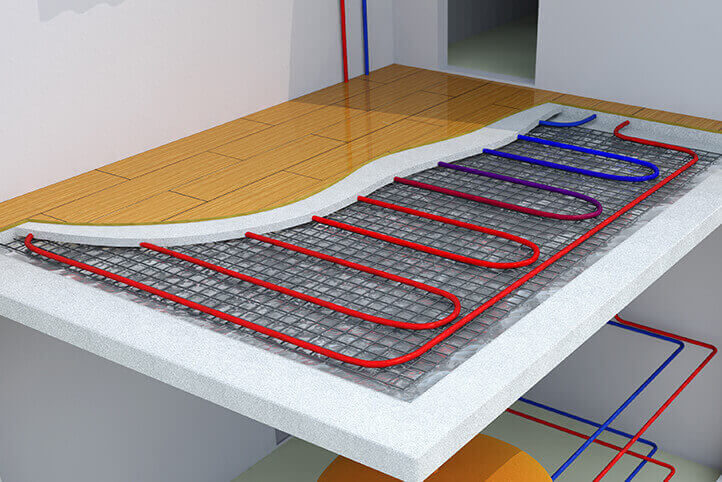
\includegraphics[width=1\textwidth]{./capitulos/resultados_discusion/images/radiant_heating_floor.jpg}
	\caption{Suelo radiante. Fuente: \url{https://www.palodurohardwoods.com/blog/radiant-heat/}}
	\label{fig:radiant_heating_floor}
\end{figure}

El suelo calienta la habitación (el aire de la habitación) principalmente por
radiación y en menor medida por convección natural, despreciándose la
transferencia de calor por conducción.

De forma que el aire de la casa también tiene una inercia térmica, y pierde
calor por las paredes, tejado y ventanas.

Las ecuaciones del balance térmico del suelo y habitación por tanto también
están acopladas y son:

\begin{align} \label{eq:floor_energy_conservation}
	m_{suelo} \cdot cp_{suelo} \cdot \left( \frac{dT_{suelo}}{dt} \right) & = \dot{Q}_{conduccion-suelo} \nonumber \\
	                                                                      & - \dot{Q}_{conveccion-suelo} \nonumber \\
	                                                                      & - \dot{Q}_{radiacion-suelo}
\end{align}

\begin{align} \label{eq:room_energy_conservation}
	m_{aire} \cdot cp_{aire} \cdot \left( \frac{dT_{habitacion}}{dt} \right) & = \dot{Q}_{conveccion-suelo} \nonumber                                     \\
	                                                                         & + \dot{Q}_{radiacion-suelo} \nonumber                                      \\
	                                                                         & - U_{paredes} \cdot A_{paredes} \cdot (T_{habitacion} - T_{amb}) \nonumber \\
	                                                                         & - U_{techo} \cdot A_{techo} \cdot (T_{habitacion} - T_{amb}) \nonumber     \\
	                                                                         & - U_{ventanas} \cdot A_{ventanas} \cdot (T_{habitacion} - T_{amb})
\end{align}

donde la transferencia de calor por conducción desde el agua caliente que
circula por los tubos hasta el suelo de hormigón viene dada por:

\begin{align} \label{eq:q_conduccion_1}
	\dot{Q}_{conduccion-suelo} & = \dot{m}_{cale} \cdot cp_{agua} \cdot (T_{tanque} - T_{cale})
\end{align}
\begin{align} \label{eq:q_conduccion_2}
	\dot{Q}_{conduccion-suelo} & = U_{tubos} \cdot A_{tubos} \cdot \Delta T_{tubos}
\end{align}

la diferencia de temperaturas representativa $\Delta T_{tubos}$ para un
intercambiador de calor sin cambios de fase se suele tomar como el LMTD (Log
Mean Temperature Difference):

\begin{equation} \label{eq:lmtd}
	\Delta T_{tubos} = \frac{(T_{tanque} - T_{suelo-salida}) - (T_{cale} - T_{suelo-entrada})}{\ln\left(\frac{T_{tanque} - T_{suelo-salida}}{T_{cale} - t_{suelo-entrada} } \right) }
\end{equation}

pero en nuestro caso hemos tomado que la temperatura del suelo se mantiene
constante a lo largo del recorrido de los tubos (figura
\ref{fig:floor_temperatures}). Esto se asemeja más al caso de un intercambiador
de calor con cambio de fase, y por tanto hemos tomado la diferencia de
temperaturas media como la representativa:

\begin{equation} \label{eq:mean_delta_T}
	\Delta T_{tubos} = \frac{(T_{tanque} - T_{suelo}) + (T_{cale} - T_{suelo})}{2}
\end{equation}

\begin{figure}[h] \centering
	\centering
	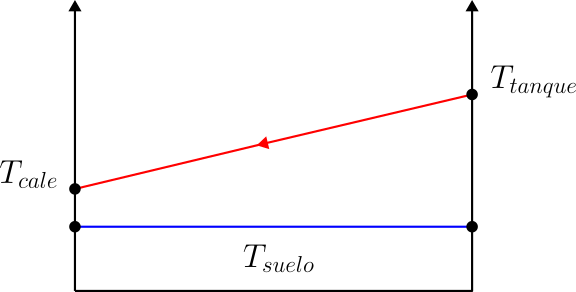
\includegraphics[width=0.6\textwidth]{./capitulos/resultados_discusion/images/floor_temperatures.png}
	\caption{Evolución de temperaturas para el suelo radiante.}
	\label{fig:floor_temperatures}
\end{figure}

y $U_{tubos}$ es la transmitancia térmica, que se considera constante para todo
el tramo del interambiador de calor, y es igual a:

\begin{equation}
	U_{tubos} = \frac{1}{\left( \frac{1}{\frac{k_{pex}}{t_{tubo}}} \right) + \left( \frac{1}{h_{tubo}} \right)}
\end{equation}

donde

\begin{itemize}
	\item $k_{pex}$: coeficiente de conductividad térmica del polietileno reticulado (PEX), igual a $0.41\left[ \frac{W}{m \cdot K} \right]$.
	\item $t_{tubo}$: Grosor del tubo de $0.635[cm]$ para tubo PEX de una pulgada.
	\item $h_{tubo}$: Coeficiente de pelicula para la transferencia de calor por convección entre el agua y los tubos.
\end{itemize}

y a su vez el coeficiente de película $h_{tubo}$ lo averiguamos del número de
Nusselt, y la ecuación de Dittus-Boelter \eqref{eq:dittus-boelter} que
relaciona los números de Prandtl, Reynolds y el Nusselt en flujo turbulento
para tubos circulares (encontrada en Incropera et al.
\cite{incropera1996fundamentals}). De forma que también suponemos que estaremos
siempre en régimen turbulento.

\begin{align}
	\text{Nu}_{tubo} & = \frac{h_{tubo} \cdot D_{tubo}}{k_{agua}}                                                                                   \\
	\text{Nu}_{tubo} & = 0.023 \cdot \text{Re}_{tubo}^{0.8} \cdot \text{Pr}_{agua}^{0.3}     \label{eq:dittus-boelter}                              \\
	\text{Re}_{tubo} & = \frac{D_{tubo} \cdot v \cdot \rho_{agua}}{\mu_{agua}} = \frac{4 \cdot \dot{m}_{cale}}{\pi \cdot \mu_{agua} \cdot D_{tubo}}
\end{align}

teniendo

\begin{itemize}
	\item $D_{tubo}$: diámetro interior del tubo de PEX.
	\item $k_{agua}$: conductividad térmica del agua a 300 Kelvin, igual a $0.6\left[\frac{W}{m \cdot K}\right]$.
	\item $\text{Pr}_{agua}$: Prandtl para el agua a 300 Kelvin. Valor de 6.9 adimensional.
	\item $v$: Velocidad del agua por los tubos.
	\item $\rho_{agua}$: densidad del agua a $300[K]$, de aproximadamente $1000\left[\frac{kg}{m^3}\right]$.
	\item $\mu_{agua}$: viscosidad dinámica del agua a $320[K]$, valiendo $0.000577[Pa \cdot s]$.
\end{itemize}


Y las transferencias de calor por radiación y convección natural de las
ecuaciones \eqref{eq:floor_energy_conservation} y
\eqref{eq:room_energy_conservation}, son:

\begin{align} \label{eq:q_radiacion}
	\dot{Q}_{radiacion-suelo} & =  \sigma \cdot \epsilon_{hormigon} \cdot A_{suelo} \cdot (T_{suelo}^4 - T_{habitacion}^4)
\end{align}

\begin{align} \label{eq:q_conveccion}
	\dot{Q}_{conveccion-suelo} & = h_{suelo} \cdot A_{suelo} \cdot (T_{suelo} - T_{habitacion})
\end{align}

con los coeficientes:

\begin{itemize}
	\item $\sigma$: constante de Stefan-Boltzmann: $5.67\cdot 10^{-8} \left[\frac{W}{m^2 \cdot K^4}\right]$.
	\item $\epsilon_{hormigon}$: emisividad del hormigón a 300 Kelvin de 0.93 (adimensional).
	\item $A_{suelo}$: superficie del suelo, $100[m^2]$.
\end{itemize}

y el coeficiente de película $h_{suelo}$ de transferencia de calor por
convección natural entre el suelo y aire de la habitación lo obtenemos
igualmente por el Nusselt, y la relación empírica
\eqref{eq:empirical_nu_natural_convection} para placas horizontales (dada en
Cengel et al. \cite{cengel2007transferencia}):

\begin{align}
	\text{Nu}_{suelo} & = \frac{h_{suelo} \cdot L}{k_{aire}} \label{eq:h_suelo}                                 \\
	\text{Nu}_{suelo} & = 0.15 \cdot \text{Ra}_{aire}^{\frac{1}{3}}  \label{eq:empirical_nu_natural_convection} \\
	\text{Ra}_{aire}  & = \text{Gr}_{aire} \cdot \text{Pr}_{aire}                                               \\
	\text{Gr}_{aire}  & = \frac{g \cdot \beta \cdot ( T_{suelo} - T_{habitacion} ) \cdot L^3}{\nu_{aire}^2}
\end{align}


donde

\begin{itemize}
	\item $\text{Nu}$: número de Nusselt.
	\item $\text{Gr}$: número de Rayleigh.
	\item $\text{Gr}$: número de Grashof.
	\item $L$: longitud característica, relación entre el área del suelo y su
	      perímetro, igual al ancho del área del suelo para planta cuadrada
	      ($10[m]$).
	\item $k_{aire}$: conductividad térmica del aire a 300 Kelvin, $0.0263\left[ \frac{W}{m \cdot K} \right]$.
	\item $g$: aceleración de la gravedad, $9.8\left[\frac{m}{s^2}\right]$
	\item $\beta$: coeficiente de expansión volumétrica para el aire, que
	      tratamos como un gas ideal a $300[K]$, y por tanto calculamos como $\beta =
		      \frac{1}{T} = \frac{1}{300} \left[K^{-1}\right]$.
	\item $\nu_{aire}$: viscosidad cinemática del aire a 300 Kelvin: $15.89 \cdot 10^{-6} \left[\frac{m^2}{s}\right]$.
\end{itemize}


\section{Simulación del sistema térmico}
\subsection{Sistema de ecuaciones reducido}

Queremos reorganizar las ecuaciones obtenidas previamente para obtener un
sistema más reducido, con menos variables de estado y control.

Para ello, primero podemos introducir \eqref{eq:q_cond_1} y \eqref{eq:q_cond_2}
en \eqref{eq:cop_t_cond}, para tener:

\begin{equation}
	\text{cop}(T_{cond}) \cdot P_{bomba} - \dot{m}_{cond} \cdot cp_{agua} \cdot \left(T_{cond} - T_{tanque}\right) = 0
\end{equation}

Por otro lado, sustituyendo \eqref{eq:m_dot_tanque} y \eqref{eq:q_perdida} en
la ecuación del balance de energía para el depósito
\eqref{eq:t_tanque_balance}, queda:

\begin{align}
	m_{tanque} \cdot cp_{agua} \cdot \left( \frac{dT_{tanque}}{dt} \right) & - \dot{m}_{cond} \cdot cp_{agua} \cdot T_{cond} \nonumber                      \\
	                                                                       & - \dot{m}_{cale} \cdot cp_{agua} \cdot T_{cale} \nonumber                      \\
	                                                                       & + (\dot{m}_{cond} + \dot{m}_{cale}) \cdot cp_{agua} \cdot T_{tanque} \nonumber \\
	                                                                       & + U_{tanque} \cdot A_{tanque} \cdot (T_{tanque} - T_{amb}) \nonumber           \\
	                                                                       & = 0
\end{align}


E insertando las expresiones para las tasas de calor por conducción, radiación
y convección del suelo radiante \eqref{eq:q_conduccion_1},
\eqref{eq:q_radiacion} y \eqref{eq:q_conveccion} respectivamente, en las
fórmulas \eqref{eq:q_conduccion_2}, \eqref{eq:floor_energy_conservation}, y
\eqref{eq:room_energy_conservation}, resultan:


\begin{align}
	\dot{m}_{cale} \cdot cp_{agua} \cdot \left(T_{tanque} - T_{cale}\right)  & - U_{tubos} \cdot A_{tubos} \cdot \Delta T_{tubos} \nonumber                                         \\
	                                                                         & = 0 \label{eq:m_cale_delta_t}                                                                        \\
	m_{suelo} \cdot cp_{suelo} \cdot \left( \frac{dT_{suelo}}{dt} \right)    & - \dot{m}_{cale} \cdot cp_{agua} \cdot (T_{tanque} - T_{cale})                             \nonumber \\
	                                                                         & + h_{suelo} \cdot A_{suelo} \cdot (T_{suelo} - T_{habitacion})                             \nonumber \\
	                                                                         & + \sigma \cdot \epsilon_{hormigon} \cdot A_{suelo} \cdot (T_{suelo}^4 - T_{habitacion}^4)  \nonumber \\
	                                                                         & = 0                                                                                                  \\
	m_{aire} \cdot cp_{aire} \cdot \left( \frac{dT_{habitacion}}{dt} \right) & - h_{suelo} \cdot A_{suelo} \cdot (T_{suelo} - T_{habitacion})  \nonumber                            \\
	                                                                         & - \sigma \cdot \epsilon_{hormigon} \cdot A_{suelo} \cdot (T_{suelo}^4 - T_{habitacion}^4)  \nonumber \\
	                                                                         & + U_{paredes} \cdot A_{paredes} \cdot (T_{habitacion} - T_{amb}) \nonumber                           \\
	                                                                         & + U_{techo} \cdot A_{techo} \cdot (T_{habitacion} - T_{amb}) \nonumber                               \\
	                                                                         & + U_{ventanas} \cdot A_{ventanas} \cdot (T_{habitacion} - T_{amb}) \nonumber                         \\
	                                                                         & = 0
\end{align}

También, de \eqref{eq:m_cale_delta_t} y \eqref{eq:mean_delta_T}, podemos despejar $T_{cale}$.

\begin{equation} \label{eq:t_cale}
	T_{cale} = \frac{2 \cdot A_{tubos} \cdot U_{tubos} \cdot T_{suelo} - A_{tubos} \cdot U_{tubos} \cdot T_{tanque} + 2 \cdot \dot{m}_{cale} \cdot cp_{agua} \cdot T_{tanque}}{A_{tubos} \cdot U_{tubos} + 2 \cdot \dot{m}_{cale} \cdot cp_{agua}}
\end{equation}

De forma que nuestro sistema finalmente consiste de:

\begin{align}
	\text{cop}(T_{cond}) \cdot P_{bomba}                                     & - \dot{m}_{cond} \cdot cp_{agua} \cdot \left(T_{cond} - T_{tanque}\right) \nonumber                  \\
	                                                                         & = 0 \label{eq:sys_1}                                                                                 \\
	m_{tanque} \cdot cp_{agua} \cdot \left( \frac{dT_{tanque}}{dt} \right)   & - \dot{m}_{cond} \cdot cp_{agua} \cdot T_{cond} \nonumber                                            \\
	                                                                         & - \dot{m}_{cale} \cdot cp_{agua} \cdot T_{cale} \nonumber                                            \\
	                                                                         & + (\dot{m}_{cond} + \dot{m}_{cale}) \cdot cp_{agua} \cdot T_{tanque} \nonumber                       \\
	                                                                         & + U_{tanque} \cdot A_{tanque} \cdot (T_{tanque} - T_{amb}) \nonumber                                 \\
	                                                                         & = 0 \label{eq:sys_2}                                                                                 \\
	m_{suelo} \cdot cp_{suelo} \cdot \left( \frac{dT_{suelo}}{dt} \right)    & - \dot{m}_{cale} \cdot cp_{agua} \cdot (T_{tanque} - T_{cale})                             \nonumber \\
	                                                                         & + h_{suelo} \cdot A_{suelo} \cdot (T_{suelo} - T_{habitacion})                             \nonumber \\
	                                                                         & + \sigma \cdot \epsilon_{hormigon} \cdot A_{suelo} \cdot (T_{suelo}^4 - T_{habitacion}^4)  \nonumber \\
	                                                                         & = 0  \label{eq:sys_3}                                                                                \\
	m_{aire} \cdot cp_{aire} \cdot \left( \frac{dT_{habitacion}}{dt} \right) & - h_{suelo} \cdot A_{suelo} \cdot (T_{suelo} - T_{habitacion})  \nonumber                            \\
	                                                                         & - \sigma \cdot \epsilon_{hormigon} \cdot A_{suelo} \cdot (T_{suelo}^4 - T_{habitacion}^4)  \nonumber \\
	                                                                         & + U_{paredes} \cdot A_{paredes} \cdot (T_{habitacion} - T_{amb}) \nonumber                           \\
	                                                                         & + U_{techo} \cdot A_{techo} \cdot (T_{habitacion} - T_{amb}) \nonumber                               \\
	                                                                         & + U_{ventanas} \cdot A_{ventanas} \cdot (T_{habitacion} - T_{amb}) \nonumber                         \\
	                                                                         & = 0  \label{eq:sys_4}
\end{align}

donde $T_{cale}$ sale de \eqref{eq:t_cale}, y $h_{suelo}$ de \eqref{eq:h_suelo}.


\subsection{Resolución con euler implícito y Newton-Raphson}

Con las igualdades \eqref{eq:sys_1}, \eqref{eq:sys_2},
\eqref{eq:sys_3}, y \eqref{eq:sys_4}, tenemos un sistema de 4
ecuaciones para 4 incógnitas: $T_{cond}$, $T_{tanque}$, $T_{suelo}$
y $T_{habitacion}$. Teniendo 4 variables de control: $\dot{m}_{cond}$,
$\dot{m}_{cale}$, $P_{bomba}$ y $T_{amb}$, aunque realmente la temperatura
ambiente no sea una variable que podamos controlar.

Se trata de ecuaciones diferenciales algebraicas (DAE,
Differential Algebraic Equation), donde solo \eqref{eq:sys_1} es algebraica,
siendo el resto diferenciales.

De índice diferencial 1, porque podemos diferenciar una vez \eqref{eq:sys_1}
para obtener $\frac{dT_{cond}}{dt}$, convirtiéndose en un conjunto de
ecuaciones diferenciales ordinarias.

Y no lineal, al tener presente la fórmula $\text{cop}(T_{cond})$ en
\eqref{eq:sys_1}, que a pesar de ser lineal a tramos, es no-lineal en su
conjunto.

La estrategia seguida para la resolución ha sido discretizar con un método
implícito, en este caso hemos optado por el método de Euler hacia atrás
(backward Euler), y en cada paso resolvemos el sistema de ecuaciones
no-lineales algebraicas resultantes con Newton-Raphson.

Recordando que la discretización con Euler implícito de un modelo ejemplo como

\begin{equation}
	\frac{dy}{dt} = f(y, t)
\end{equation}

corresponde a

\begin{equation}
	\frac{y_k - y_{k-1}}{h} = f(y_k, t_k)
\end{equation}

donde $h$ es el paso empleado.

Nuestro sistema reducido se presenta de la siguiente forma:

\begin{align}
	\text{cop}(T_{cond,k}) \cdot P_{bomba,k}                                                    & - \dot{m}_{cond,k} \cdot cp_{agua} \cdot \left(T_{cond,k} - T_{tanque,k}\right) = 0                     \\
	m_{tanque} \cdot cp_{agua} \cdot \frac{\left(T_{tanque,k} - T_{tanque,k-1}\right)}{h}       & - \dot{m}_{cond,k} \cdot cp_{agua} \cdot T_{cond,k} \nonumber                                           \\
	                                                                                            & - \dot{m}_{cale,k} \cdot cp_{agua} \cdot T_{cale} \nonumber                                             \\
	                                                                                            & + (\dot{m}_{cond,k} + \dot{m}_{cale,k}) \cdot cp_{agua} \cdot T_{tanque,k} \nonumber                    \\
	                                                                                            & + U_{tanque} \cdot A_{tanque} \cdot (T_{tanque,k} - T_{amb,k}) \nonumber                                \\
	                                                                                            & = 0                                                                                                     \\
	m_{suelo} \cdot cp_{suelo} \cdot \frac{\left(T_{suelo,k} - T_{suelo,k-1}\right)}{h}         & - \dot{m}_{cale,k} \cdot cp_{agua} \cdot (T_{tanque,k} - T_{cale}) \nonumber                            \\
	                                                                                            & + h_{suelo} \cdot A_{suelo} \cdot (T_{suelo,k} - T_{habitacion,k}) \nonumber                            \\
	                                                                                            & + \sigma \cdot \epsilon_{hormigon} \cdot A_{suelo} \cdot (T_{suelo,k}^4 - T_{habitacion,k}^4) \nonumber \\
	                                                                                            & = 0                                                                                                     \\
	m_{aire} \cdot cp_{aire} \cdot \frac{\left(T_{habitacion,k} - T_{habitacion,k-1}\right)}{h} & - h_{suelo} \cdot A_{suelo} \cdot (T_{suelo,k} - T_{habitacion,k}) \nonumber                            \\
	                                                                                            & - \sigma \cdot \epsilon_{hormigon} \cdot A_{suelo} \cdot (T_{suelo,k}^4 - T_{habitacion,k}^4) \nonumber \\
	                                                                                            & + U_{paredes} \cdot A_{paredes} \cdot (T_{habitacion,k} - T_{amb,k}) \nonumber                          \\
	                                                                                            & + U_{techo} \cdot A_{techo} \cdot (T_{habitacion,k} - T_{amb,k}) \nonumber                              \\
	                                                                                            & + U_{ventanas} \cdot A_{ventanas} \cdot (T_{habitacion,k} - T_{amb,k}) \nonumber                        \\
	                                                                                            & = 0
\end{align}


\subsection{Simulación}


En python, empleamos la rutina `fsolve` del paquete `scipy.optimize` para
resolver el sistema discretizado a cada paso con Newton-Raphson.

\begin{minted}{python}
def solve(y_0, u, dae_p, h, n_steps):
    """
    Solve the differential-algebraic equation (DAE) system using implicit time-stepping.

    Parameters:
    y_0: Initial conditions of the states.
    u: Control inputs over time.
    dae_p: Parameters for the DAE system.
    h: Time step size.
    n_steps: Number of time steps to perform.

    Returns:
    y:  State evolution over time.
    """
    # Initialize solution
    y = np.zeros((len(y_0), n_steps))

    # Initial conditions
    y[:, 0] = y_0

    # Time-stepping loop
    for n in range(1, n_steps):
        # Use fsolve to solve the nonlinear system
        y_n = fsolve(dae_system, y[:, n - 1], args=(y[:, n - 1], u[:, n], dae_p, h))
        y[:, n] = y_n

    return y
\end{minted}

y la función \textit{dae\_system} a su vez recibe el estado actual, previo,
variables de control actuales, parámetros y paso, y devuelve el valor de las
ecuaciones, con todos los términos en un mismo miembro.


\begin{minted}{python}
def dae_system(y, y_prev, u, p, h):
		# Here we name all variables from y, y_prev, u and p:
		# ...

    h_floor_air = get_h_floor_air(
        t_floor,
        t_room,
        gravity_acceleration,
        air_volumetric_expansion_coeff,
        floor_width,
        nu_air,
        Pr_air,
        k_air,
        A_roof,
    )

    h_tube_water = get_h_tube_water(
        tube_inner_diameter,
        mu_water_at_320K,
        Pr_water,
        k_water,
        m_dot_heating,
    )

    U_tubes = 1 / ((1 / h_tube_water) + (1 / (k_pex / tube_thickness)))

    t_out_heating = (
        2 * A_tubes * U_tubes * t_floor - A_tubes * U_tubes * t_tank + 2 * cp_water * m_dot_heating * t_tank
    ) / (A_tubes * U_tubes + 2 * cp_water * m_dot_heating)

    return [
        # 1
        cop(t_cond) * p_compressor - m_dot_cond * cp_water * (t_cond - t_tank),
        # 2
        m_tank * cp_water * ((t_tank - t_tank_prev) / h)
        - m_dot_cond * cp_water * t_cond
        - m_dot_heating * cp_water * t_out_heating
        + (m_dot_cond + m_dot_heating) * cp_water * t_tank
        + U_tank * A_tank * (t_tank - t_amb),
        # 3
        floor_mass * cp_concrete * ((t_floor - t_floor_prev) / h)
        - m_dot_heating * cp_water * (t_tank - t_out_heating)
        + h_floor_air * floor_area * (t_floor - t_room)
        + stefan_boltzmann_constant * epsilon_concrete * floor_area * (t_floor**4 - t_room**4),
        # 4
        room_air_mass * cp_air * ((t_room - t_room_prev) / h)
        - h_floor_air * floor_area * (t_floor - t_room)
        - stefan_boltzmann_constant * epsilon_concrete * floor_area * (t_floor**4 - t_room**4)
        + U_walls * A_walls * (t_room - t_amb)
        + U_roof * A_roof * (t_room - t_amb)
        + U_windows * A_windows * (t_room - t_amb),
    ]
\end{minted}

Probamos a simular este modelo aplicando un paso de $100[s]$, condiciones iniciales:

\begin{align}
	T_{cond_0} = 296.56[K]       \\
	T_{tanque_0} = 296.05[K]     \\
	T_{suelo_0} = 295.27[K]      \\
	T_{habitacion_0} = 293.47[K] \\
\end{align}

y los siguientes controles:

\begin{equation}
	\dot{m}_{cond}(t)[kg \cdot s^{-1}] =
	\begin{cases}
		0.3 & \text{si } 0 \leq t < \frac{3T}{4},            \\
		0.1 & \text{si } \frac{3T}{4} \leq t < \frac{5T}{6}, \\
		0.3 & \text{si } \frac{5T}{6} \leq t \leq T.
	\end{cases}
\end{equation}

\begin{equation}
	\dot{m}_{cale}(t)[kg \cdot s^{-1}] =
	\begin{cases}
		0.2 & \text{si } 0 \leq t < \frac{T}{2},            \\
		0.1 & \text{si } \frac{T}{2} \leq t < \frac{4T}{5}, \\
		0.2 & \text{si } \frac{4T}{5} \leq t \leq T.
	\end{cases}
\end{equation}

\begin{equation}
	P_{bomba}(t)[W] =
	\begin{cases}
		300                                                      \\
		1 \cdot 10^{-6} & \text{si } \frac{2T}{3} \leq t \leq T.
	\end{cases}
\end{equation}

$T$ siendo el periodo de simulación de 7 días, y $T_{amb}$ la temperatura
ambiente para estos.

El resultado se aprecia en la figura \ref{fig:simulacion_1}.
Donde el primer gráfico muestra la evolución de las temperaturas,
mantiéndose siempre

\begin{equation*}
	T_{cond} > T_{tanque} > T_{suelo} > T_{habitacion}
\end{equation*}

En la segunda ilustración vemos las tasas de calor por transferencia de calor
por conducción (de los tubos a la losa de suelo), y por radiación y convección
natural, del suelo al aire de la habitación.

El suelo principalmente calienta por radiación, y la aportación por
convección es alrededor de un tercio de esta.

Cuando la losa de hormigón recibe más calor del agua de la calefacción
(conducción) que evacúa en la habitación, observamos su temperatura aumentar.
Para más claridad se ha representado la suma de los términos convectivo y
radiativo.

En las dos últimas gráficas aparecen las variables de control empleadas: los
caudales dirigidos a la calefacción del suelo radiante, y de la bomba de calor
al tanque de agua, y la potencia destinada a la bomba de calor (o compresor de
esta).

Para ambos, es visible que hemos aplicados funciones escalón para estimular al
sistema.

\begin{figure}[h] \centering
	\centering
	\includesvg[width=1\textwidth]{./capitulos/resultados_discusion/images/simulacion_1}
	\caption{Simulación del sistema térmico con paso $h=100[s]$.}
	\label{fig:simulacion_1}
\end{figure}


El paso $h$ empleado en las simulaciones debe ser lo suficientemente pequeño
como para poder representar las dinámicas más rápidas del sistema. Estas
dinámicas las observamos al aplicar una función escalón en los controles del
modelo. Y reducimos progresivamente el tamaño del paso hasta que la solución
converja.

En este caso tenemos una respuesta lenta, debido a las inercias térmicas de
tanto depósito, como suelo radiante y habitación. De modo que hemos empleado en
lo siguiente un paso de 1000 segundos, al no apreciar diferencia en los
resultados que se arrojan (figura \ref{fig:simulacion_2_h:1000}), y así no tenemos la necesidad de considerar tantas
variables de diseño en nuestros estudios de control óptimo, donde a cada paso
elegimos qué caudales y potencia destinar a la bomba de calor.

\begin{figure}[h] \centering
	\centering
	\includesvg[width=1\textwidth]{./capitulos/resultados_discusion/images/simulacion_2_h:1000s}
	\caption{Temperaturas del sistema térmico con paso $h=1000[s]$.}
	\label{fig:simulacion_2_h:1000}
\end{figure}

Tampoco usamos un paso mayor que este porque el sistema eléctrico con el que
vamos a optimizar conjuntamente el sistema, tiene una dinámica horaria
(precios, potencias solares dadas por los paneles y demanda eléctrica del
domicilio se dan horariamente), y es recomendable usar un paso alrededor de un order
de magnitud menor que la dinámica más rápida.

En el extremo donde se dan respuestas muy rápidas y también muy lentas, se
habla de un sistema rígido, en referencia de un péndulo con un periodo
asociado, pero que además tiene otra oscilación mucho más rápida en su cuerpo,
que puede modelarse como un resorte rígido (figura \ref{fig:stiff_system}). El
problema que existe en estas circunstancias es que para simular el
comportamiento del péndulo, debemos de usar un paso muy pequeño, del orden de
la velocidad del resorte rígido, lo que puede llevar a costes computacionales
muy grandes en la simulación.

\begin{figure}[h] \centering
	\centering
	\includesvg[width=0.3\textwidth]{./capitulos/resultados_discusion/images/stiff_system}
	\caption{Sistema rígido.}
	\label{fig:stiff_system}
\end{figure}


\section{Optimizacion del control}

con derivadas adjuntas y SAND, comparar
10 dias

\subsection{Derivadas adjuntas}
\subsection{SAND}

aqui vemos que SAND es superior a MDF, en caso de ser viable su uso,
y por tanto a partir de ahora estudiamos solo el uso de SAND


\section{Optimizacion del control y dimensionamiento}
\subsection{Autoconsumo con compensación simplificada}
- 30 dias (no tenemos bateria virtual)
- dimensionamiento con media ponderada

- 365 dias (tenemos bateria virtual, pero no merece la pena acumular en un año, suponiendo que todos los años son iguales más o menos)
- 365 dias con C-rate de 1

no es realista suponer que tenemos conocimiento perfecto de precios futuros.
realmente tendriamos que optimizar nuestro sistema con nuestra estimacion
de precios, como con una red neural, aunque en este trabajo no se cubre este caso.

\subsection{Sistema off-grid}

\subsection{Libre venta de electricidad a precio de mercado}

\section{Valoracion de impactos}
